\chapter{Área de Estudo}
A área de estudo está localizada na bacia hidrográfica do rio São João (BHRSJ) Figura \ref{fig:locareaestudo}. Esta bacia hidrográfica localiza-se na região das Baixadas Litorâneas do estado do Rio de Janeiro, interior à Área de Proteção Ambiental da bacia do rio São João/Mico-Leão-Dourado, e é uma das principais contribuintes da Represa de Juturnaíba. A BHRSJ está situada dentro do contexto da Mata Atlântica entra a Serra do Mar e o litoral atlântico e posiciona-se à oeste da Bacia Hidrográfica da Baía da Guanabara, estendendo-se por 63 km no sentido leste-oeste e por 43 km no sentido norte-sul, e possuindo uma área total de 2.160 km2. O mesmo nasce a 800m de altitude, no município de Cachoeiras de Macacu, num trecho da serra do Mar conhecido como serra do Sambê. Possui cerca de 120 km de comprimento e deságua no oceano entre a vila de Barra de São João, na margem esquerda, e o povoado de Santo Antônio, que pertence a Cabo Frio, na margem direita. Suas paisagens, ao longo dos últimos 500 anos, foram intensamente modificadas com o processo de desmatamento do bioma originário Mata Atlântica, com fins de implantação de atividades agropastoris e, a partir dos anos de 1960, de forma pontual com as obras nas planícies aluviais realizadas pelo extinto DNOS (Departamento Nacional de Obras e Saneamento). \\

	\begin{figure}
		\centering
		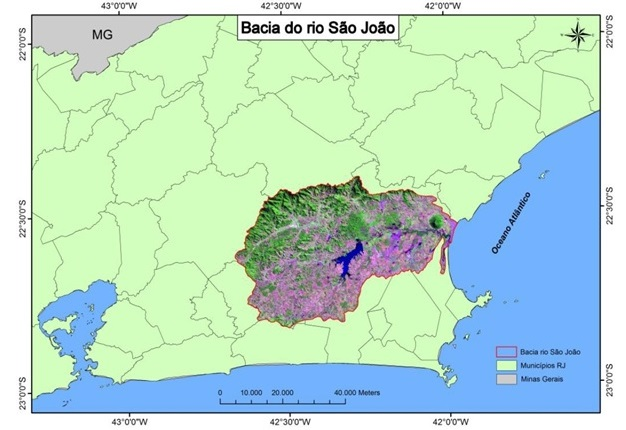
\includegraphics[width=0.9\linewidth]{C:/Users/eduardo/Documents/Projetos/TeX/mestrado/data/BHRSJ.jpg}
		\caption{Localização da área de estudo.}
		\label{fig:locareaestudo}
	\end{figure}


A partir das obras do DNOS com a retilinização dos canais, problemas sedimentológicos foram gerados devido a diminuição da retenção da água, causando a erosão das margens. Além disso, houveram problemas relacionados ao alagamento de certas localidades e o consequente abandono das mesmas. \\

	\begin{figure}
		\centering
		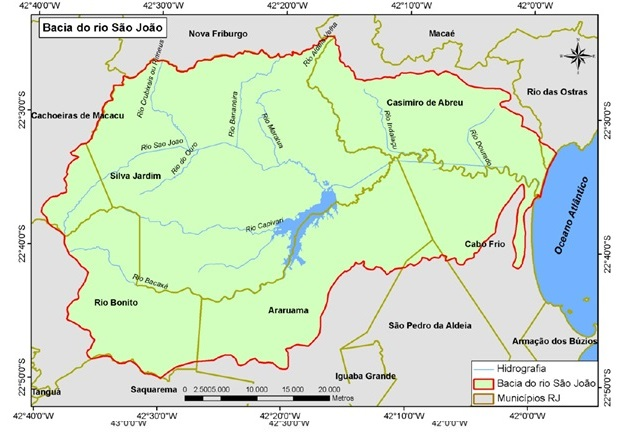
\includegraphics[width=0.9\linewidth]{data/BHRSJ_2}
		\caption{Municípios inseridos na Bacia do rio São João.}
		\label{fig:bhrsj2}
	\end{figure}


A BHRSJ possui ainda um contexto ambiental no qual vem apresentando uma taxa de recuperação florestal devido ao posicionamento das áreas degradadas perto de áreas de cobertura vegetal, o que vem favorecendo tal recuperação como demonstrado por Seabra \& Cruz (2013) \cite{SEABRA_CRUZ}. Tais características favorecem ainda mais a escolha da BHRSJ como uma área para um estudo de caso no trabalho proposto aqui. \\
